%% ============================================================
%%  MLIR 的多级抽象设计及其在 AI 编译器生态中的角色
%%  CS323 Compilers —— Research Report (Fall 2026)
%%
%%  编译引擎：XeLaTeX（含中文，pdfLaTeX 不可用）
%%  编译顺序：xelatex -> bibtex -> xelatex -> xelatex
%%  格式：acmsmall（ACM 期刊小号单栏；不是 sigconf 双栏会议版）
%% ============================================================
%% nonacm=true 是 acmart 的官方开关，用于"非 ACM 出版"场合：会去掉首页的版权块、
%% 价格行与虚构 DOI（否则会出现 "2026. 0164-0925/... $15.00" 与 doi.org/10.1145/nnnn...）。
%% 注意 acmart 的 toppmatter 只有 printccs / printacmref / printfolios 三个键，
%% 没有 printcopyright，所以不能靠 \settopmatter 关版权块。
\documentclass[acmsmall, screen=true, nonacm=true]{acmart}

%% ---- 期刊信息 ----
%% acmart 的 \acmJournal 是 xkeyval 的 choice key：只接受其内部注册的代码。
%% 写成 CS323 之类的自定义名称会直接报 "Class acmart Error: Incorrect journal"。
%% 本文按主题选用 TOPLAS（ACM Transactions on Programming Languages and Systems）。
%% 其它常用合法代码：TACO / TOMS / CSUR / TOPC。
\acmJournal{TOPLAS}
\acmYear{2026}
\acmVolume{1}
\acmNumber{1}
\acmArticle{1}
\acmMonth{11}
\setcopyright{none}

%% ---- 中文支持 ----
%% 本文含中文，必须用 XeLaTeX 或 LuaLaTeX 编译。pdfLaTeX 会报
%%   "Unicode character 的 (U+7684) not set up for use with LaTeX"
%% Overleaf：Menu -> Settings -> Compiler -> XeLaTeX
\usepackage{iftex}
\ifPDFTeX
  \PackageError{main}{This report contains Chinese text.^^J%
    Switch the compiler to XeLaTeX (or LuaLaTeX) and recompile.}%
    {Overleaf: Menu -> Settings -> Compiler -> XeLaTeX}
\fi
\ifXeTeX
  \usepackage{xeCJK}
  \setCJKmainfont[ItalicFont=FandolKai-Regular.otf,BoldFont=FandolHei-Regular.otf]{FandolSong-Regular.otf}
  \setCJKsansfont[AutoFakeBold=2]{FandolHei-Regular.otf}
  \setCJKmonofont{FandolFang-Regular.otf}
\fi
\ifLuaTeX
  \usepackage{luatexja-fontspec}
  \setmainjfont{FandolSong-Regular.otf}
  \setsansjfont{FandolHei-Regular.otf}
  \setmonojfont{FandolFang-Regular.otf}
\fi

%% ---- 表 1 需要；图用 graphicx（acmart 已加载） ----
\usepackage{booktabs}
\usepackage{tabularx}
\usepackage{amsmath}
\usepackage{siunitx}
%% SVG 图：Overleaf 自带 inkscape，可启用下面这行并把 \includegraphics 换成 \includesvg
%% \usepackage{svg}

%% ---- 关闭版权块与 ACM Reference Format 占位 ----
%% 课程报告不投 ACM，避免出现虚构 DOI/版权声明。
%% 注意：不要用 \def\footnotetextcopyrightpermission#1{} 之类的重定义 ——
%% acmart 是用 {…\par…} 调它的，非 \long 的 \def 会报
%% "Paragraph ended before \footnotetextcopyrightpermission was complete"。
%% 官方做法是 \setcopyright{none}（copyright mode = none 会同时关掉 copyright 与 permission）。
\settopmatter{printacmref=false}
\pagestyle{plain}

%% 中文断行没有连字符可拆，遇到 \texttt{...} 这类不可断的长串容易溢出；
%% 放宽一排版的伸缩余量，消掉 Overfull \hbox。
\setlength{\emergencystretch}{2em}

\begin{document}

\title{MLIR 的多级抽象设计及其在 AI 编译器生态中的角色：\\从成对适配到分层共享的复用成本分析}

%% ---- 作者信息（按需填写学号） ----
\author{Su-dum}
\affiliation{%
  \institution{Southern University of Science and Technology}
  \department{Department of Computer Science and Engineering}
  \city{Shenzhen}
  \country{China}}
\email{12410337@mail.sustech.edu.cn}

\author{（组员姓名，待填）}
\affiliation{%
  \institution{Southern University of Science and Technology}
  \city{Shenzhen}
  \country{China}}

\renewcommand{\shortauthors}{Su-dum et al.}

%% ============================================================
\begin{abstract}
%% TODO(§ 摘要)：定稿时写成三句——问题与通行叙事（N×M）、本文做法（重构命题 + 语料实证 + 成本模型）、
%% 结论的限定形式（"在……条件下成立"）。以下是占位草稿，不要原样提交。
一个编译器要同时面对 $N$ 个前端框架与 $M$ 种硬件，逐对适配的成本是乘法的。
本文把"MLIR 解决了 $N\times M$ 组合爆炸"这一通行叙事，重构为一个可检验的命题：
MLIR 把适配成本从 $N\cdot M$ 重写为 $|E|+N+M$，但收益取决于共享层是否被多方采纳。
基于 \texttt{llvm-project} 的 3,329 个 MLIR 测试文件（181,326 个算子），
本文测得 $|E|=76$ 条方言间转换、$371$ 个转换文件中有 $298$ 个进入层间矩阵，并发现收敛发生在少数端点上而非层级上。
成本模型显示，工程层面的门槛约在 9 到 26 个前端之间（随采纳率），而架构层面的门槛只有约 5 个。
\end{abstract}

%% ---- CCS Concepts：若需完整版，请从 dl.acm.org 的 CCS 工具生成 CCSXML 后粘贴 ----
%% （不提供 CCSXML 也能编译；下面只给 \ccsdesc 会正常排出版块）
\begin{CCSXML}
<ccs2012>
 <concept>
  <concept_id>10011007.10011006.10011041</concept_id>
  <concept_desc>Software and its engineering~Compilers</concept_desc>
  <concept_significance>500</concept_significance>
 </concept>
 <concept>
  <concept_id>10011007.10011006.10011008</concept_id>
  <concept_desc>Software and its engineering~Intermediate languages</concept_desc>
  <concept_significance>300</concept_significance>
 </concept>
</ccs2012>
\end{CCSXML}
\ccsdesc[500]{Software and its engineering~Compilers}
\ccsdesc[300]{Software and its engineering~Intermediate languages}

\keywords{MLIR, multi-level IR, dialect, progressive lowering, AI compiler, reuse cost}

\maketitle

%% ============================================================
%% ============================================================
%%  §1 引言
%%  要证明的一句话：
%%    一层 IR 通吃的假设（源自同构 CPU 时代）在"多框架 × 异构加速器"下失效，
%%    本文把这个失效重述为一个可检验的成本结构问题。
%%  素材：docs/01-outline-v1.md §1（四个必答问题）
%%  建议篇幅：1.5 页
%% ============================================================

\section{引言}
\label{sec:intro}

%% TODO(问题陈述)：不要用"随着深度学习的发展"开头。
%% 直接从算账开始：一个编译器要同时面对 K 个前端与 J 个后端，逐对适配的成本是乘法的。
%% 必须给出具体数字（N 与 M），每一处数字配脚注来源。

%% TODO(为什么一层不够)：引用 §2 的结论——每个系统都固定在某一层，而固定点越低前端越厚、
%% 越高后端越厚（表 1）。所以"选一层"是权衡，不是可以回避的问题。

%% TODO(本文命题)：写成可被推翻的形式。
%% 关键：不要说"MLIR 解决了 N×M"。

%% TODO(贡献三条)：
%% ① 把 N×M 叙事重构为"成本重分配 + 条件性收益"；
%% ② 用 MLIR 自身测试语料量化层间结构（|E| = 76，且是下界）；
%% ③ 给出可代入的成本模型与交叉点 N*，并做 p 的敏感性分析。

%% TODO(不做什么)：不做性能评测、不评判框架优劣、不覆盖全部 LLVM 生态。

%% ---- 图 1：成本模型（立问题） ----
%% 说明：单栏模式下 figure 已是整栏宽，可直接用 \linewidth。
%% 用 PNG 先保证能编译；确认无误后可改用 \includesvg{figures/fig3_cost_model}。
\begin{figure}[t]
  \centering
  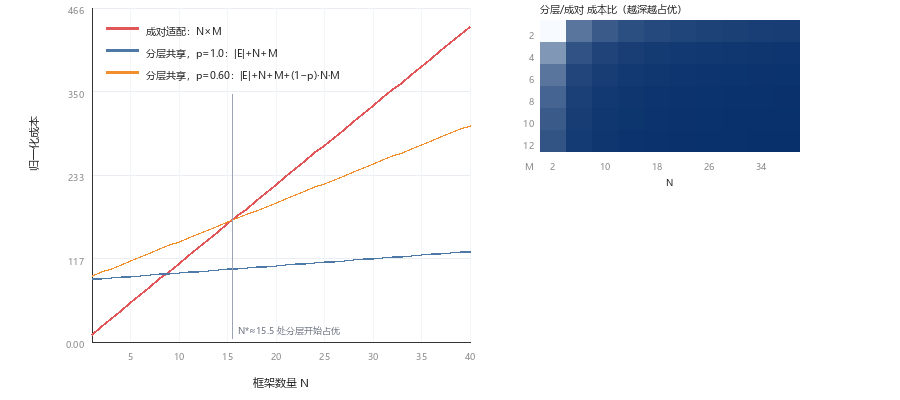
\includegraphics[width=\linewidth]{figures/fig3_cost_model.png}
  \caption{成本随规模的变化。实线为成对适配 $N\cdot M$；虚线为分层共享
  $|E|+N+M+(1-p)\cdot N\cdot M$（$|E|=76$，$M=11$，$p=0.6$）。
  竖虚线为交叉点 $N^\ast\approx15.5$。右图为 $(N,M)$ 平面上的成本比。}
  \Description{左图为三条成本曲线与交叉点，右图为成本比热力图}
  \label{fig:cost}
\end{figure}

%% ============================================================
%%  §2 只选一层的代价：从 LLVM IR 到 XLA 与 Triton
%%  要证明的一句话：
%%    每个系统都把抽象层固定在某处；固定点越低则前端越厚、后端越薄，反之亦然。
%%    这是权衡曲线，不是优劣排序。
%%  素材：docs/05-section2-comparison.md
%% ============================================================

\section{只选一层的代价}
\label{sec:background}

\ref{sec:intro} 节把问题重述为"适配成本如何组织"。在讨论 MLIR 之前，需要先回答一个更基本的问题：
在 MLIR 出现之前，业界是如何选"那一层"的？本节考察五个代表性系统，只描述它们把抽象固定在哪里、
硬件知识从哪个口子进入，不做优劣判断——因为"选哪一层"本身是受使用场景约束的权衡，
而不是有唯一正确答案的设计题。

\subsection{五个系统，五种固定方式}

\paragraph{LLVM IR：把硬件知识整体推迟}
LLVM 的目标无关 SSA 中间表示在设计上就假定自己不含目标细节~\cite{llvm04}，
三地址码、标量或向量指令与显式内存语义构成其基本单位。硬件知识并非不存在，而是被
\textbf{整体推迟}到 IR 之后：指令选择、调度与 MC 层。因此扩展一个新后端，等于实现一套
\texttt{TargetLowering} 与指令选择模式；扩展一个新前端，则需要把源语言的全部语义下降成 LLVM IR。

\paragraph{Halide：把调度从算法里拆出来}
Halide 的核心贡献是算法与调度的解耦~\cite{halide12,halide13}：同一份算法可以配不同调度
（tile、vectorize、parallel），再配不同后端；官方支持 x86、ARM、MIPS、Hexagon、PowerPC、
RISC-V，以及 CUDA、OpenCL、OpenGL Compute、Metal、DirectX~12。这实际上是"把硬件知识外置成
调度"的早期形态，也是后来 \texttt{linalg} 的 structured operations 与 transform dialect 的思想来源。

\paragraph{TVM：固定两层}
TVM 同时暴露图级与算子级优化~\cite{tvm18}：图级负责算子融合等粗粒度变换，算子级负责
"映射到任意硬件原语"，并把内存延迟隐藏交给调度。硬件知识主要进入\textbf{算子级}——通过
tensor intrinsic、内存布局与 target 相关的下放规则。固定两层的好处是图级优化不必关心目标，
代价是接入新硬件往往要同时适配两层。

\paragraph{XLA：固定一层，其余交给后端}
XLA 的流程是三段式~\cite{xlaarch}：先在 StableHLO 上做\textbf{目标无关}的优化并转成内部
HLO；再交给后端做\textbf{目标相关}的 HLO 级优化；最后生成 LLVM IR 交给 LLVM 完成代码生成。
值得单独指出的是，布局（layout）在 HLO 内部就以显式 pass 的形式被指派~\cite{xlathunks}——
XLA 把"数据在内存里怎么摆"这件与硬件强相关的事，放在了与 IR 同一层处理。新增后端的路径是
"实现 \texttt{xla::Compiler} 接口"~\cite{xlabackend}。

XLA 官方文档自己给出了这个设计的动机，原话是：\emph{retargeting XLA should be significantly
simpler and more scalable than implementing every existing op from a frontend framework such as
PyTorch or TensorFlow for new hardware}~\cite{xlabackend}。这句话很重要：它说明"避免逐对适配"
不是本文事后附会的叙事，而是项目自己写下的设计目标。于是本文的问题不是新造的——同一问题上，
XLA 与 MLIR 给了两种不同的答案。

\paragraph{Triton：固定 tile 级，并且本身就是 MLIR 的一组方言}
Triton 面向分块（tiled）的神经网络计算~\cite{triton19}，把抽象固定在一块张量上，配合显式的
grid 模型。它常被误解为"绕开通用编译栈"的例子，但其编译器\textbf{本身就构建在 MLIR 上}：
其 IR 是一组方言，\texttt{tt}（Triton IR）$\rightarrow$ \texttt{ttg}（TritonGPU，含布局）
$\rightarrow$ \texttt{ttng}/\texttt{nvg}（NVIDIA）或 \texttt{amdg}（AMD）~\cite{tritondialects}。
换句话说，Triton 是 MLIR 的一种\textbf{纵向用法}——只保留必要的一两级方言，把 tile 级钉死，
再一路下到厂商方言；它与 IREE、StableHLO 这类"宽栈"用法共同构成 MLIR 生态的两种形态。

\begin{table}[t]
  \caption{各系统把抽象层固定在何处，以及硬件知识与新前端的进入点。}
  \label{tab:layer-fixing}
  \small
  \begin{tabularx}{\linewidth}{@{}l
      >{\raggedright\arraybackslash}p{1.5cm}
      >{\raggedright\arraybackslash}p{1.9cm}
      >{\raggedright\arraybackslash}p{1.7cm}
      >{\raggedright\arraybackslash}p{1.9cm}
      >{\raggedright\arraybackslash}p{1.3cm}@{}}
    \toprule
    系统 & 固定的抽象层 & 硬件知识进入点 & 新增前端 & 新增后端 & 复用单位 \\
    \midrule
    LLVM IR & 一层：目标无关 SSA IR & 指令选择、调度、MC 层
      & 生成 LLVM IR & 实现 TargetLowering / ISel & pass \\
    Halide & 一层：算法 + 调度 & 调度原语与后端
      & 写算法（内嵌 DSL） & 接入一个后端 & 调度原语 \\
    TVM & 两层：图级 + 算子级 & 算子级调度与 target 下放
      & 导入为图级 IR & target 描述 + codegen / BYOC & 调度原语 \\
    XLA & 一层：HLO & HLO 内部 pass 与后端重写
      & 生成 StableHLO & 实现 \texttt{Compiler} 接口 & HLO pass \\
    Triton & 一层：tile 级 & tile 布局（\texttt{ttg}）与厂商方言
      & 生成 tile 级程序 & 厂商方言 + lowering & dialect \\
    MLIR & \textbf{不固定} & 任意 dialect 边界
      & 定义前端 dialect & 定义目标 dialect + 转换 & dialect / 转换 \\
    \bottomrule
  \end{tabularx}
\end{table}

\subsection{三点评注}

\paragraph{一：层的位置是守恒的，不是可以省掉的}
表中六行没有一行是"无层"的——每行都选了至少一层，TVM 选了两层。能变的只是"选在哪"。
因此严格的说法不是"有了 MLIR 就不必选层"，而是：\textbf{抽象层的位置可以随域调整，
但抽象层的总量不会消失}。MLIR 改变的是"谁来做这个选择、以及能否在同一程序里保留多个选择"，
而不是"可以不做选择"。

\paragraph{二：固定点越低，前端越厚、后端越薄——这是一条权衡曲线}
LLVM IR 固定在最低处：前端必须承担全部语义下降，后端只需做指令选择；XLA 固定在高处：
前端只需产出 StableHLO（极薄），后端必须承担全部目标相关重写（极厚）。Halide、TVM、Triton
落在曲线的不同高度上。

这条曲线与 \ref{sec:intro} 的成本模型直接咬合：\textbf{最优固定点由 $N$ 与 $M$ 的相对大小决定}。
若一个系统预期被很多前端复用、只服务少数后端，把层压低更划算；反之应把层抬高。
这个判断与具体技术优劣无关，只与生态规模有关。

\paragraph{三：XLA 与 MLIR 是同一问题的两种答案，差别在"谁承担不确定性"}
两者都以"避免为每个硬件重写全部算子"为动机（前者见上引 XLA 原文，后者见 MLIR 的
\emph{software fragmentation}~\cite{mlir21}）。差别在于不确定性被放在哪里：XLA 把它收进后端，
以换取 HLO 这一层的稳定；MLIR 把它放到 dialect 边界上，允许边界本身被重新协商。

这一区别不需要评判谁更好，但它解释了第~\ref{sec:evidence} 节的实证结果：如果 MLIR 的成功
取决于"边界能否被协商成功"，那么\textbf{边界协商的成本}就是关键变量——这正是第~\ref{sec:contract} 节
要考察的内容。

\paragraph{关于表~\ref{tab:layer-fixing} 的 MLIR 一行}
该行是\textbf{机制描述}（依据 MLIR 的设计文献与官方文档），不是本文的实测结果；
它与第~\ref{sec:evidence} 节基于语料统计的证据强度不同，不应等同看待。

%% ============================================================
%%  §3 MLIR 的机制：层级如何变成一等对象
%% ============================================================

\section{机制：层级如何变成一等对象}
\label{sec:mechanisms}

上节说明每个系统都必须选层。MLIR 的特别之处不在于它"层更多"，而在于它\textbf{不把层的数量与
位置写进框架的前提}。本节只讨论撑起这一点的四个机制，不逐一介绍 MLIR 有哪些方言，那属于手册而不是论证。

\subsection{机制一：dialect 把"一层"搬到库边界}

一个 dialect 打包的是\textbf{一整套}设施：算子集合、类型与属性、验证规则，
以及可定制的打印/解析与规范化行为~\cite{mlir21}；这些由 ODS（Operation Definition
Specification）在构建期生成~\cite{mlirods}。

这一点常被低估。若"新增一层"意味着修改编译器内核（新增 IR 节点种类、改遍历与重写框架），
那么每加一层都要付内核级成本，层的数量必然稀缺；而 dialect 让这一整包东西成为
\textbf{可插拔的库单元}：新增一层不必改内核，只需链接一个库并注册。

\subsection{机制二：多级共存与部分下降}

MLIR 允许不同抽象高度的算子在同一个 module 里共存，且都是合法 IR。这不是实现细节，
而是"渐进下降"（progressive lowering）的前提：若层级不能共存，下降就只能整段一次性完成，
"分层"随即退化为"分阶段流水线"，复用单位也重新变成整条流水线。

图~\ref{fig:mixed-levels} 用真实语料把这一点变得可见。同一个文件里有两个函数：\texttt{@matmul}
用一次 \texttt{linalg.matmul} 表达整个矩阵乘，没有显式循环；\texttt{@matvec} 中同一计算已经
被显式化为 \texttt{scf.for} 循环加子算子 \texttt{linalg.matvec}。两者共存于同一 module 且都能
通过验证。由此可推出三件事：下降可以是\textbf{部分的}；层的边界是工程决策而非合法性约束；
因此最小复用单位可以是一条转换。

这条结论将在第~\ref{sec:evidence} 节被量化：正是因为它成立，"方言对"才能成为一个有意义的
成本计数单位。

\subsection{机制三：op interface 是可加性的技术根源}

这是本节最容易被写浅的一处。常见的表述是"interface 让不同 dialect 共享同一套操作"，
这既不准确也不够有力。真正起作用的是：\textbf{一条转换可以只依赖 interface 而不依赖具体方言，
因此不必为新方言重写}~\cite{mlirinterfaces}。

举例来说，tiling、fusion 这类变换只需要目标算子满足"可被切分"的接口约定，而不关心它是
\texttt{linalg.matmul} 还是某个厂商的私有算子。于是生态里新增一个方言时，已有变换往往可以
直接复用，这是 $N+M$ 而非 $N\times M$ 的技术根据。反过来，若没有 interface，每加一个方言
就要为每个变换写一遍适配，成本立刻退回乘法。

\subsection{机制四：conversion target 与 legality 让边界可声明}

层与层之间的边界在 MLIR 里是\textbf{可声明}的：conversion target 指明哪些
算子与类型在目标层合法，legality 规则据此判定"下降是否完成"，type converter 负责跨层的类型映射
~\cite{mlirconversion}。这使得"边界"本身成为可检验对象，可以问"这一步之后还有哪些非法算子
残留"，而不必靠人工判断"看起来下降完了"。

代价也是真实的：一条链上 pass 的顺序变得敏感，不完整的下降容易留下难以定位的残留。
这一点与 bufferization、shape 推断的困难一起，在第~\ref{sec:limitations} 节讨论。

\begin{figure}[t]
  \centering
  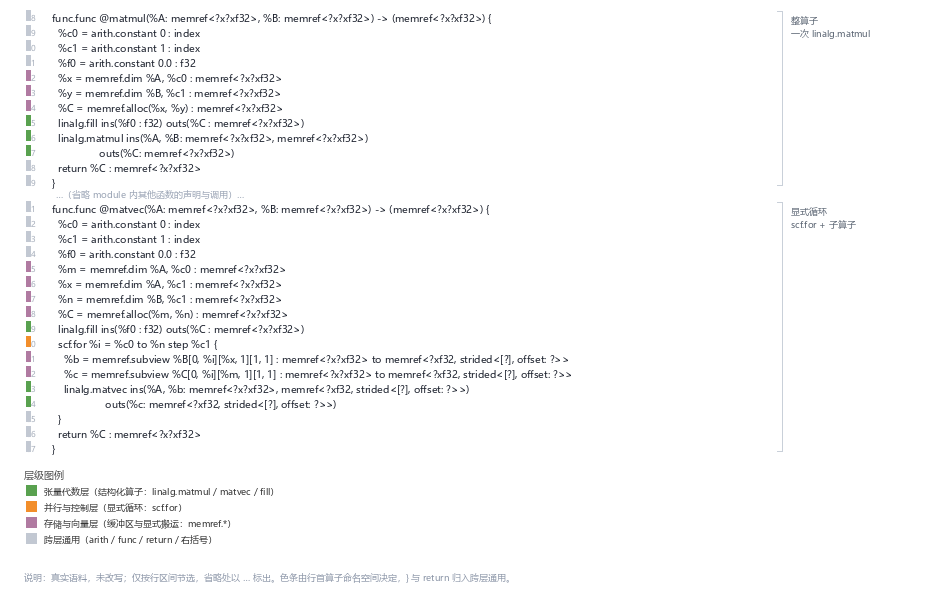
\includegraphics[width=\linewidth]{figures/fig_mixed_levels.png}
  \caption{同一 module 内的多级抽象共存。选自 \texttt{llvm-project@ba736172} 的
  \texttt{mlir/test/Integration/Dialect/Linalg/CPU/matmul-vs-matvec.mlir}，节选 29 行，未改写；
  左侧色条标出该行算子所属的抽象层。\texttt{@matmul} 以单个 \texttt{linalg.matmul} 表达
  整个矩阵乘；\texttt{@matvec} 中同一计算已被显式化为 \texttt{scf.for} 循环与子算子
  \texttt{linalg.matvec}。两者共存于同一 module，说明下降可以是部分的。}
  \Description{带层级色条的 MLIR 代码片段，两个函数分别使用整算子与显式循环}
  \label{fig:mixed-levels}
\end{figure}

\subsection{小结：机制的作用范围}

四个机制合起来说明：MLIR 不预设层数，其设施使层的划分可被协商。但这些机制只保证层可以被重新划定，
机制只保证"层可以被重新划定"，不保证"某一层会被多方采纳"。后者是生态问题，需要成本证据
（第~\ref{sec:evidence} 节）与治理证据（第~\ref{sec:contract} 节）才能回答。

第~\ref{sec:evidence} 节的实证正由这两个机制直接支撑：方言对之所以能作为可数的成本单位，
靠的是机制二（部分下降使单条转换有意义）与机制三（interface 使单条转换可跨方言复用）。

%% ============================================================
%%  §4 生态结构实证
%%  要证明的一句话：
%%    在上游语料中，转换强度收敛于少数"端点"而非层级；成本随硬件家族数增长，
%%    因此"塌缩"在架构层几乎立即发生，在工程层需要十几个到二十几个前端。
%%  素材：docs/04-results-v1.md（五条发现 + 稳健性检验）
%%  建议篇幅：3.5 页（含图 3、图 4、表 2）
%% ============================================================

\section{生态结构实证}
\label{sec:evidence}

%% ---- 方法段（必须先写，且必须交代口径） ----
%% 数据：llvm-project@ba736172 的 mlir/test/**，3329 个 .mlir，181326 个算子。
%% 单元：Conversion/<X>To<Y> 目录 -> 一条层间边；452 个转换文件中 371 个可解析，
%%       81 个因一端方言不定被排除（故 |E| 是下界）。
%% 层划分：5 层 + 跨层通用方言；划分是主观的，已做替代划分的稳健性检验。
%% 一句话必须写：本节统计的是"测试文件数量"，是工程投入分布的代理指标，不是性能、不是使用率。

%% ---- 发现 1：收敛在端点，不在层 ----
%% 79.2% 的层间转换落到最深层（236/298）；但真正的汇聚点是方言：
%% llvm 入度 104、来自 19 个不同方言；其次 rocdl 57、spirv 57。
%% 结论句：共享不是层与层的对称交换，而是所有源指向少数终端的星形结构。
\begin{figure}[t]
  \centering
  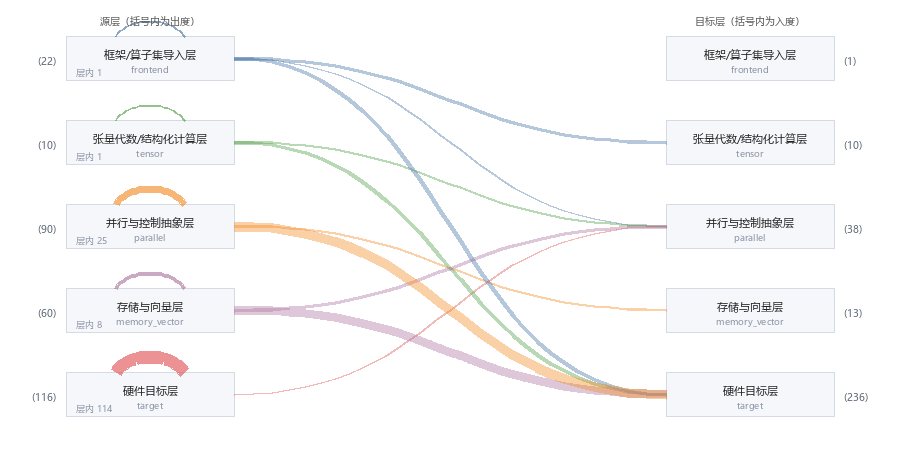
\includegraphics[width=\linewidth]{figures/fig1_layer_transitions.png}
  \caption{层间转换强度（按抽象层聚合）。线宽正比于该层间转换对应的
  \texttt{Conversion} 测试文件数；弧线自左（源层）指向右（目标层）。
  汇入最深层的那束粗线即"端点收敛"。}
  \Description{五层之间的转换弧线图，最右一列入度最大}
  \label{fig:transitions}
\end{figure}

%% ---- 发现 2：厂商在 MLIR 里占两级，不是一层 ----
%% target→target 有 114 个文件 / 8 条边，是全部层间转换中最大的一块：
%% 厂商内二级栈（amdgpu→rocdl 42、xegpu→xevm 20、nvgpu→nvvm 6）与出口转向（spirv→llvm 25 等）。
%% 归因要谨慎：厂商内二级栈只有 3 条边（68 个文件），不是 15→76 膨胀的主因；
%% 主因是层边界内部本身含多个方言对（一条边界平均约 5 个）。

%% ---- 发现 3：投入"两级结构、前端独低"（表 2） ----
\begin{table}[t]
  \caption{各抽象层的测试投入分布。按 \texttt{test/Dialect/<X>} 归属到层；
  跨层通用方言与编译器基础设施方言单列。已归属文件共 1,390 个。}
  \label{tab:investment}
  \small
  \begin{tabularx}{\linewidth}{@{}l S[table-format=3.0] S[table-format=2.1]@{}}
    \toprule
    层 & {文件数} & {占已归属（\%）} \\
    \midrule
    硬件目标层 & 364 & 26.2 \\
    张量代数/结构化计算层 & 354 & 25.5 \\
    并行与控制抽象层 & 235 & 16.9 \\
    存储与向量层 & 222 & 16.0 \\
    跨层通用方言（单列） & 73 & 5.3 \\
    编译器基础设施方言（6 个，单列） & 80 & 5.8 \\
    \textbf{框架/算子集导入层} & \textbf{62} & \textbf{4.5} \\
    \bottomrule
  \end{tabularx}
\end{table}

%% 解释：分布是明显两级——高档（目标 26.2%、张量 25.5%）、中档（并行 16.9%、存储 16.0%）、
%% 低档（导入 4.5%）。导入层只有中后段的约 1/4–1/6。
%% 注意：v1 曾写"四个中后段层几乎均匀（20.6–24.0%）"，那是 Dialect/SparseTensor 与
%% Dialect/LLVMIR 被静默丢弃导致的，已按 review 修正。
%% 原因：承接框架的活在别的仓库（torch-mlir、StableHLO、ONNX-MLIR）；
%% 本语料里 frontend 层作为转换源的方言只有 tosa，torch/stablehlo 一个都没有。

%% ---- 发现 4：两种 |E| 口径，答案相反 ----
%% 架构级 15 个层对 -> N* = 4.6；工程级 76 个方言对 -> N* = 15.5（p=0.6, M=11）。
%% 在 N=8、M=11 时：成对 88 vs 分层 69.2（架构级占优）；88 vs 130.2（工程级更贵）。
%% 敏感性：p 从 1.0 降到 0.4，N* 从 8.7 升到 25.6（约 2.9 倍）。
%% 结论形式必须带条件，不能写成"MLIR 让成本塌缩"。

%% ---- 发现 5：func / arith 是唯一的真·跨层通用语（图 4） ----
\begin{figure}[t]
  \centering
  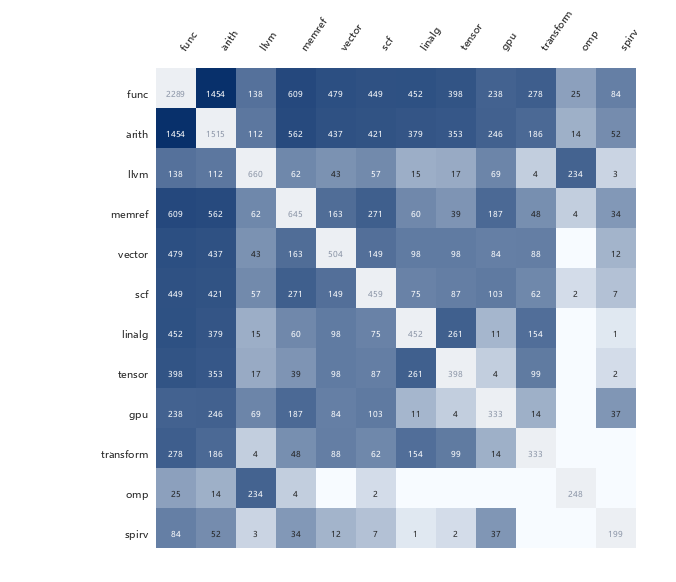
\includegraphics[width=\linewidth]{figures/fig2_dialect_cooccurrence.png}
  \caption{方言共现矩阵（同一测试文件内同时出现）。取文档频次最高的 12 个方言；
  非对角格为双方的共现文件数，颜色取对数刻度；对角线灰格为该方言自身的文档频次，
  量纲不同，不参与色阶。\texttt{func}/\texttt{arith} 与几乎所有层都共现，
  印证其"跨层通用语"地位。}
  \Description{12x12 的方言共现热力图}
  \label{fig:cooccurrence}
\end{figure}

%% ---- 稳健性检验（必须有，证明做过证伪） ----
%% 替代划分（target 拆成通用出口 + 厂商方言，5→6 层）：
%% |E| = 76 与工程级 N* 完全不变；"落到最深层"从 79.2% 掉到 36.6%；非零层对 15→20。
%% 结论：方言级数字是稳的，层级的百分比是划分依赖的 —— 正文只用前者。

%% ============================================================
%%  §5 共享契约的谈判成本：mhlo -> StableHLO
%%  要证明的一句话：
%%    把一个方言变成各方都敢依赖的契约，需要版本化、序列化与兼容测试等制度性设施；
%%    这部分成本不体现在 |E| 里，却决定共享层采纳率 p 能否上去。
%%  素材：docs/07-section5-stablehlo.md
%%  建议篇幅：1.5 页
%% ============================================================

\section{共享契约的谈判成本}
\label{sec:contract}

%% 开篇：§3 说明了 MLIR 有能力让层被协商，但没说明"协商成功"需要什么。
%% 本节用一个真实的迁移案例回答。

%% ---- MHLO 的位置问题 ----
%% 它长期作为独立孵化仓库存在于 tensorflow/mlir-hlo，定位是"独立于 TF 与 XLA 的端到端流程"、
%% "把技术上游化的孵化器"。把它当框架与编译器之间的接口，等于把跨组织接口放在一个项目的内部 IR 上。
%% 现状：官方已标 deprecated，建议迁移（措辞是 deprecated + 迁移建议，不是"设计不好"）。

%% ---- StableHLO 的增量：全是契约设施，不是算子语义 ----
%% 官方自述："基于 MHLO，并增加了序列化与版本化"，以此提供前后向兼容保证。
\begin{table}[t]
  \caption{StableHLO 相对 MHLO 增加的契约设施。新增项均为"制度性"机制，
  而非算子语义改造。}
  \label{tab:contract}
  \small
  \begin{tabularx}{\linewidth}{@{}l X@{}}
    \toprule
    机制 & 具体做法 \\
    \midrule
    定位 & 明确充当 ML 框架与编译器之间的 portability layer \\
    序列化 & portable artifact 用 MLIR bytecode；CLI / C++ / Python 三种入口 \\
    版本号 & \texttt{\#.\#.\#}：minor 随 opset 或序列化格式变更递增；patch 随发布递增，每周一次 \\
    不可回填 & 版本被 supersede 后不能再添加内容，变更必须开新 minor（旧版本语义被冻结） \\
    VHLO & 把"版本化"本身做成一个方言；序列化时 StableHLO $\rightarrow$ 目标版本的 VHLO \\
    兼容窗口 & \textbf{5 年向后兼容} + \textbf{2 年向前兼容} \\
    CI 门槛 & 每个 PR 都测双向兼容；目标版本取至少 4 / 12 周前被 supersede 的版本 \\
    显式排除 & prettyprinted IR、未规格化特性、bug compatibility 均\textbf{不}保证 \\
    \bottomrule
  \end{tabularx}
\end{table}

%% ---- 三条推论 ----
%% A. 契约的成本是治理成本：上表没有一行是"再实现一个算子"；成本在 RFC、每周发版、
%%    一个 VHLO 方言、逐 PR 的兼容测试套。
%% B. 这套治理能力不在 MLIR 里：compatibility.md 的 Future work 明确说要"把兼容性测试套
%%    贡献回 MLIR 上游"（issue #1632）。在贡献之前，契约是 StableHLO 自己立法、自己执行、自己承担。
%%    => 这正是 §4 结论"收益条件性"的机制解释：MLIR 提供机制，契约由采用者建立。
%% C. 契约必须显式排除才能成立：out-of-scope 三条说明"边界可声明，但不等于边界免费"，
%%    接得上 §3 的机制 ④。

%% 收束句（建议原话）：
%% 由此可见，MLIR 让层可被协商，但把某一层变成各方都敢依赖的契约，需要采用者自建版本、
%% 序列化与兼容测试制度；这部分成本不体现在转换数量 |E| 里，却决定了 p 能否真正上去。

%% ============================================================
%%  §6 代价、局限与威胁效度
%% ============================================================

\section{代价、局限与威胁效度}
\label{sec:limitations}

本节做两件事：先说清这套设计的\textbf{代价}（属于 MLIR，不属于本文方法），再说清本文证据
\textbf{能支撑到哪一步}，并把结论按强度分级。

\subsection{机制层面的代价}

\paragraph{栈顶仍然碎片化}
第~\ref{sec:evidence} 节的投入分布显示，导入层只占已归属文件的 4.5\%，而承接框架的工作分散在
\texttt{torch-mlir}、StableHLO、\texttt{onnx-mlir} 等\textbf{不同仓库}里。共享的收益并没有在栈顶
兑现，而是被推迟到了各生态自己的项目中。准确的说法不是"MLIR 没有解决框架接入"，而是
"\textbf{MLIR 把栈顶的共享收益外置给了生态}"。

\paragraph{抽象泄漏集中在三处}
层与层之间的边界并非处处等价。最难的几处是：\textbf{bufferization}~\cite{mlirbufferization}（从值语义到缓冲区语义，
每次读写都要决定 copy 还是原地改写，这是语义决策而非语法改写）、\textbf{shape 推断}~\cite{mlirshape}
（动态维度需要约束与见证的传播，语义横跨 shape、tensor、memref 三层）、\textbf{量化}
（scale 与 zero-point 的归属需要额外的类型层承载）。这类信息无法被完全抽象掉，
因此每增加一层就增加一处潜在的语义错位点。

\paragraph{pass 链变长，调试面变大}
第~\ref{sec:mechanisms} 节机制四指出边界是可声明的，代价是 pass 顺序变敏感、不完整的下降会留下
难以定位的残留。需要明确：\textbf{本文没有测量这一成本}，它只作为机制层面的定性判断存在。

\paragraph{治理成本}
第~\ref{sec:contract} 节已把这一项枚举为可数的工程产物（RFC、每周发布、VHLO、逐 PR 兼容测试）。
它不体现在 $|E|$ 里，却直接决定采纳率 $p$。

\subsection{本文实证的局限}

表~\ref{tab:threats} 逐条把局限绑定到被削弱的结论上。

\begin{table}[t]
  \caption{本文实证的局限及其对结论的影响。右列说明正文中的处理方式。}
  \label{tab:threats}
  \small
  \begin{tabularx}{\linewidth}{@{}l X X@{}}
    \toprule
    局限 & 证据 & 影响与处理 \\
    \midrule
    语料是上游测试集 & 3,329 个文件中 \texttt{Integration/*} 占 423 个（12.7\%），
      以 GPU 端到端为主 & 投入分布类结论限定为结构性描述，不作使用率推断 \\
    目标端分布不均 & 入矩阵文件的目标家族：通用 CPU 101、AMD 65、通用 GPU 57、Intel 33、
      NVIDIA 21、C/C++ 19、Arm 3，合计 299；另有 72 个落在中间层目标
      & "收敛在 \texttt{llvm}" 表述为\textbf{上游语料中}的收敛；GPU 厂商合计 119，被过度代表 \\
    $|E|$ 是接口数量的代理 & 76 条方言对；一条 \texttt{Conversion} 目录可能包含多个 pass
      & 明写等权假设；结论是结构性的，不是绝对成本 \\
    口径偏差 & \texttt{builtin} 因无命名空间被显著低估；81 个转换文件因一端方言不定被排除
      & 明写 $|E|=76$ 是\textbf{下界}，真实门槛只会更不利 \\
    层划分主观 & 主划分 15 个非零层对，替代划分 20 个；最深层占比 79.2\% $\rightarrow$ 36.6\%
      & 已做稳健性检验；正文只用划分不变量 \\
    只用一个仓库 & 未纳入 \texttt{torch-mlir}、StableHLO、\texttt{onnx-mlir} 的语料
      & 栈顶碎片化只能间接推断，列为后续工作 \\
    参数来源不对称 & $M=11$ 由数据自动实测；$N=8$ 为生态假设；$p$ 只做敏感性
      & 明写三者来源差异；结论不依赖 $p$ 的具体取值 \\
    \bottomrule
  \end{tabularx}
\end{table}

其中两条值得额外说明。

\textbf{$|E|$ 是下界，而这反而加强了结论的方向。}81 个转换文件因一端方言不定被排除，
因此真实方言对数只会比 76 更多；门槛随 $|E|$ 上升，所以工程级门槛只可能更高。
方向上对本文有利，但数值上必须如实标注为下界。

\textbf{"落到最深层"的百分比不可单独引用。}它是 79.2\%（236/298），但这个数字依赖"把硬件目标层
划成一层"这一选择；换成两层划分后掉到 36.6\%。正文因此只用方言级的量（104 个文件、19 个来源
汇入 \texttt{llvm}），不用层级的百分比。

\subsection{结论强度分级}

\textbf{硬结论}（方言级，与层划分无关，可以直接断言）：$|E|=76$（下界）；\texttt{llvm} 的入度为
104 个文件、来自 19 个方言；最深层内部 114 个文件 / 8 条边（68 个厂商内 + 46 个出口转向）；
导入层投入占比 4.5\%。

\textbf{软结论}（依赖参数或划分，必须带条件说）：工程级门槛 $N^{*}\approx 15.5$
（$M=11$、$p=0.6$）；架构级门槛 $N^{*}\approx 4.6$；采纳率敏感性约 2.9 倍。
引用时都需带上 $M$ 与 $p$ 的取值。

\textbf{不可断言}：任何性能、编译时间或使用率数字（本文没有测量）；"MLIR 解决了 $N\times M$"；
单独引用 79.2\%。

\subsection{本文的自我定位}

本文能支持的最强主张是：\textbf{MLIR 把适配成本的组织方式从成对定制改为分层共享，
并在上游语料中呈现出以 \texttt{llvm} 为端点的收敛；而这一转变的工程门槛取决于谁支付 $|E|$}。
本文不能支持的是：这一转变在具体硬件上更快，或已被多数框架采纳。

%% ============================================================
%%  §7 结论
%%  要证明的一句话（全篇落点）：
%%    能力不等于效果：MLIR 让层可协商，但收益的门槛恰好落在现实 AI 框架的数量级附近，
%%    这既解释了它近年被广泛采纳，也解释了为什么采纳不是自动发生的。
%%  建议篇幅：0.4 页
%% ============================================================

\section{结论}
\label{sec:conclusion}

%% 三段结构：
%% ① 回到命题：一句话概括本文把 N×M 叙事重构为什么。
%% ② 用数字收口：|E| = 76（下界）；收敛在端点（llvm 104 / 19 源）；门槛 4.6（架构级）
%%    到 15.5（工程级，p=0.6），敏感性 2.9 倍（8.7→25.6）。
%% ③ 落点：能力 != 效果；治理成本（§5）是 p 上不去的机制原因；
%%    由此可解释"MLIR 在 2020–2023 被广泛采纳，而更早的单层 IR 方案没有"。

%% 可选一句展望：把 torch-mlir 与 OpenXLA 的语料并入，可把"栈顶碎片化"从间接推断
%% 变成直接测量。


%% ---- 可选：AI 使用披露（课程已取消强制要求；保留与否自定） ----
%% \section*{Use of AI Tools}
%% ...

\bibliographystyle{ACM-Reference-Format}
\bibliography{references}

\end{document}
